%%%%%%%%%%%%%%%%%%%%%%%%%%%%%%%%%%%%%%%%%%%%%%%%%%%%%%%%%%%%%%%%%%%%%%%%%%%%%
% 26/05/2010
% edited by Bill Lampos
%
% Feel free to use (copy) the structure (latex formatting source code)
% but not the content of this document.
%
%%%%%%%%%%%%%%%%%%%%%%%%%%%%%%%%%%%%%%%%%%%%%%%%%%%%%%%%%%%%%%%%%%%%%%%%%%%%%
\documentclass[compress,red]{beamer}
\mode<presentation>

\usetheme{Warsaw}
%\usetheme{Darmstadt}
% other themes: AnnArbor, Antibes, Bergen, Berkeley, Berlin, Boadilla, boxes, CambridgeUS, Copenhagen, Darmstadt, default, Dresden, Frankfurt, Goettingen,
% Hannover, Ilmenau, JuanLesPins, Luebeck, Madrid, Maloe, Marburg, Montpellier, PaloAlto, Pittsburg, Rochester, Singapore, Szeged, classic

%\usecolortheme{lily}
% color themes: albatross, beaver, beetle, crane, default, dolphin, dov, fly, lily, orchid, rose, seagull, seahorse, sidebartab, structure, whale, wolverine

%\usefonttheme{serif}
% font themes: default, professionalfonts, serif, structurebold, structureitalicserif, structuresmallcapsserif

% pdf is displayed in full screen mode automatically
%\hypersetup{pdfpagemode=FullScreen}

% define your own colours:
\definecolor{Red}{rgb}{1,0,0}
\definecolor{Blue}{rgb}{0,0,1}
\definecolor{Green}{rgb}{0,1,0}
\definecolor{magenta}{rgb}{1,0,.6}
\definecolor{lightblue}{rgb}{0,.5,1}
\definecolor{lightpurple}{rgb}{.6,.4,1}
\definecolor{gold}{rgb}{.6,.5,0}
\definecolor{orange}{rgb}{1,0.4,0}
\definecolor{hotpink}{rgb}{1,0,0.5}
\definecolor{newcolor2}{rgb}{.5,.3,.5}
\definecolor{newcolor}{rgb}{0,.3,1}
\definecolor{newcolor3}{rgb}{1,0,.35}
\definecolor{darkgreen1}{rgb}{0, .35, 0}
\definecolor{darkgreen}{rgb}{0, .6, 0}
\definecolor{darkred}{rgb}{.75,0,0}

\xdefinecolor{olive}{cmyk}{0.64,0,0.95,0.4}
\xdefinecolor{purpleish}{cmyk}{0.75,0.75,0,0}

% \usepackage{beamerinnertheme_______}
% inner themes include circles, default, inmargin, rectangles, rounded

%\usepackage{beamerouterthemesmoothbars}
% outer themes include default, infolines, miniframes, shadow, sidebar, smoothbars, smoothtree, split, tree

\useoutertheme[subsection=false]{smoothbars}

% to have the same footer on all slides
%\setbeamertemplate{footline}[text line]{xxx xxx xxx}
%\setbeamertemplate{footline}[text line]{} % or empty footer

% include packages
\usepackage{subfigure}
\usepackage{multicol}
\usepackage{amsmath}
\usepackage{epsfig}
\usepackage{graphicx}
\usepackage[all,knot]{xy}
\xyoption{arc}
\usepackage{url}
\usepackage{multimedia}
\usepackage{hyperref}
\usepackage{setspace}
\usepackage{algorithm}
\usepackage[noend]{algpseudocode}
%Page number
%\setbeamertemplate{footline}[frame number]
\setbeamertemplate{sidebar right}{}
\setbeamertemplate{footline}{%
\hfill\usebeamertemplate***{navigation symbols}
\hspace{1cm}\insertframenumber{}/\inserttotalframenumber}

\title{Multiparameter resource selection for next
generation HPC platforms}
\subtitle{Master Research Thesis}
\author{Dineshkumar RAJAGOPAL}
\institute{{\tiny advised by}\\ \vspace{.10cm}Dr Yiannis GEORGIOU}
\date{\scriptsize Big Data and Security(BDS) lab, BULL-SAS\\ \vspace{.10cm}September 1, 2015}

\begin{document}

\frame{
	\titlepage
}

\section[Outline]{}
\frame{\tableofcontents}

\section{RJMS}
\subsection{Basic concepts of RJMS}
\frame{\frametitle{Basic concepts of RJMS}
\begin{enumerate}

\item The goal of a \textbf{Resource and Job Management System (RJMS)} is
to satisfy users demands for computation and \textbf{assign resources
to user jobs} with an efficient manner\\
\vspace{0.25cm}
\item \textbf{RJMS} is the system software between jobs and resources. It knows the complete details about the HPC system\\
\centering 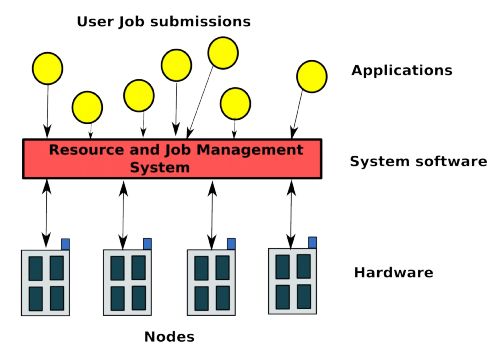
\includegraphics[scale=.4,keepaspectratio]{image/HPC-RJMS-role.png}

\end{enumerate}
}

\frame{\frametitle{HPC system software stack}
\begin{enumerate}
\item RJMS is called as \textbf{workload manager, loadleveler, batch scheduler, etc} \\
\item RJMS's strategic position in the HPC system software stack\\
\vspace{0.25cm}
\centering 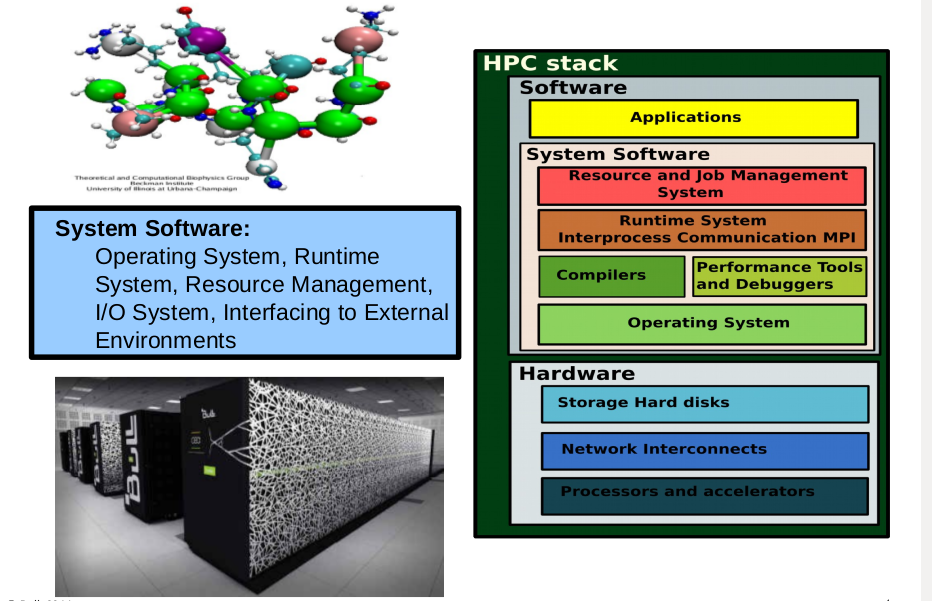
\includegraphics[scale=.25,keepaspectratio]{image/HPC-RJMS-SS.png}
\end{enumerate}
}

\section{SLURM}
%\subsection{SLURM Architecture}
%\frame{\frametitle{Being more specific}
%\begin{enumerate}
%\item \textbf{Trends} about what? Examples?
%      \begin{itemize}
%        \item Predict flu rates (\emph{epidemics})
%        \item Infer vote intensions (\emph{politics})
%        \item Infer traffic/weather conditions (\emph{toy problems})\pause
%      \end{itemize}
%\vspace{0.25cm}
%\item \textbf{Methodologies}?
%      \begin{itemize}
%        \item Feature extraction/selection
%        \item Exploit probabilistic relationships (PGMs)
%        \item Regression/classification/ranking scenarios
%        \item Active learning\pause
%      \end{itemize}
%\vspace{0.25cm}
%\item \textbf{Applications}?
%      \begin{itemize}
%        \item Back-end infrastructure for data collection/retrieval/mining
%        \item Real time online tools for making and displaying predictions (like the \href{http://geopatterns.enm.bris.ac.uk/epidemics/}{\textbf{Flu detector}})
%      \end{itemize}
%\end{enumerate}
%}
\subsection{SLURM architecture and entities}
\frame{ 
\frametitle{SLURM architecture}
\begin{enumerate}
\item SLURM$'$s high level components architecture and daemon program \\
\vspace{0.25cm}
\centering 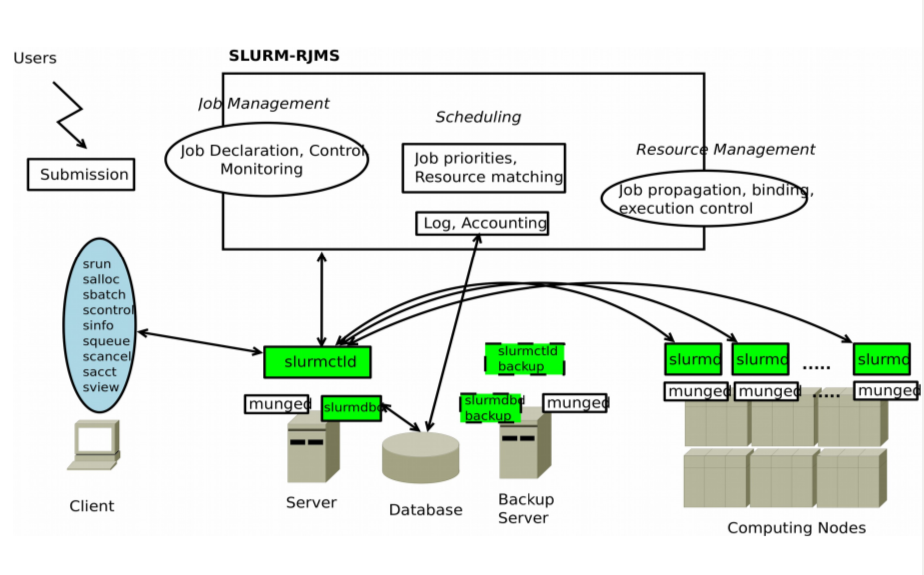
\includegraphics[scale=0.33,keepaspectratio]{image/SLURM-RJMS-Archi.png}
\end{enumerate}
}

\frame{ 
\frametitle{SLURM entities}
\begin{enumerate}
\item SLURM resource and job management entities \\
\vspace{0.5cm}
\centering 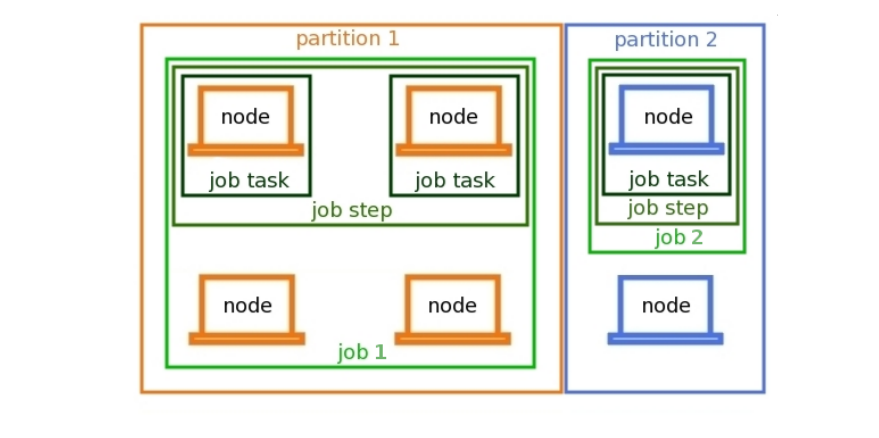
\includegraphics[scale=0.33,keepaspectratio]{image/SLURM-Entities-cropped.png}
\end{enumerate}
}

\subsection{Consumable resource selection}
\frame{ 
\frametitle{Consumable resource selection cycle}
\begin{enumerate}
\item \textbf{Cons\_res} plugin implemented the following algorithm \\
\item States(\textbf{Reject non-runnable jobs, Find nodes for job, Preempt jobs if necessary}) are the selection algorithm\\
\vspace{0.25cm}
\centering 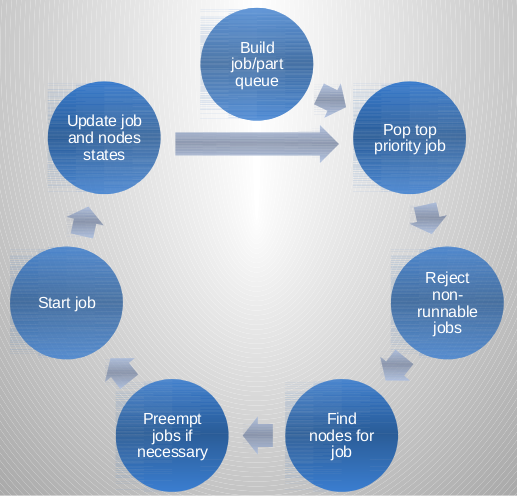
\includegraphics[scale=0.3,keepaspectratio]{image/SLURM-scedule-loop-cropped.png}
\end{enumerate}

}

\frame{ 
\frametitle{Consumable Resource Selection Algorithm}
\begin{enumerate}
\item \textbf{Bestfit} to reduce fragmentation \\
\item \textbf{Topology aware} to increase the user application performance \\
\item \textbf{Algorithm 1} in the \textbf{section 3.1} of the \textbf{report} discussed the algorithm step by step \\
\end{enumerate}

}

\section{LAYOUTS Framework}
\subsection{Internal architecture}
\frame{\frametitle{LAYOUTS Framework}
\begin{enumerate}
\item LAYOUTS is the resource management framework in SLURM \\
\vspace{0.25cm}
\item \textbf{Terminology:}
	\begin{itemize}
		\item LAYOUTS - Framework \\
		\item Layout(s) or layout(s) - Resource management plugin \\
	\end{itemize} 
\vspace{0.25cm}
\item \textbf{Physical and logical} entities can be manageable\\
\vspace{0.25cm}
\item Entity relation is \textbf{tree}\\
\vspace{0.25cm}
\item Entity attributes are called \textbf{keys} \\
\vspace{0.25cm}
\item Entity and immediate entities keys relation are defined \\
\vspace{0.25cm}
\item \textbf{Key relations} are aggregate functions(Sum, Avg, etc) following \textbf{tree relations} \\
\end{enumerate}
}

\frame{\frametitle{LAYOUTS internal architecture}
}
\frame{\frametitle{LAYOUTS entity data management}

}

\frame{\frametitle{LAYOUTS entities key and key relations}

}

\frame{\frametitle{LAYOUTS aggregate key options}

}

\subsection{LAYOUTS APIs}
\frame{\frametitle{LAYOUTS APIs}

}
\frame{\frametitle{LAYOUTS new APIs}

}

\section{Resource Selector and Improvements}
\subsection{LAYOUTS based consumable resource selection}
\frame{\frametitle{LAYOUTS plugin for cons\_res\_layout}
}

\frame{\frametitle{Resource selection policy of cons\_res\_layout}

}

\subsection{Energy efficient consumable resource selection}
\frame{\frametitle{LAYOUTS plugin for cons\_res\_power}
}

\frame{\frametitle{Resource selection policy of cons\_res\_power}

}


\section{Performance Evaluation}
\subsection{Experiment environment}
\frame{\frametitle{Experiment environment}
}

\subsection{Performance analysis}
\frame{\frametitle{LAYOUTS plugin for cons\_res\_layout}
}

\frame{\frametitle{Resource selection policy of cons\_res\_layout}

}
\section{Conclusion and Future Work}
\frame{\frametitle{Conclusion}
}

\frame{\frametitle{Future work}

}
\section*{}
\frame{
    \begin{center}
        \huge
        Thank you ..\\
        \vspace{0.25cm}
        Any questions?
    \end{center}
}

\end{document} 